\section{Emergence, Benefits and Limitations of Using Edge Computing}

\begin{table*}[t]
\begin{adjustwidth}{-2.7cm}{-1cm}
\caption{Edge Computing use cases, current limitations, and imperatives}
\label{tab:use_case}
\begin{tabular}{|c|c|c|c|}
\hline
Applications                                                                                    & Example Use Case                                                                                                                                                                              & Limitations                                                                                                                                                      & Requirements                                                                                                                                         \\ \hline
Smart City                                                                                      & \begin{tabular}[c]{@{}c@{}}Help autistic people \\ navigate through large \\ crowded spaces.\end{tabular}                                                                                     & \begin{tabular}[c]{@{}c@{}}Hard to provide real-time \\ directions due to the need to \\ send large volumes of data to \\ the cloud.\end{tabular}                & \begin{tabular}[c]{@{}c@{}}Low Latency, Security,\\ Geographically \\ Distributed,\\ Mobility, Scalability\\ Reliability and Robustness\end{tabular} \\ \hline
\begin{tabular}[c]{@{}c@{}}Disaster \\ Recovery\end{tabular}                                    & \begin{tabular}[c]{@{}c@{}}Need to quickly determine \\  whether  building conditions \\ are safe for  evacuees to return \\ after a natural  disaster \\ has struck.\end{tabular}            & \begin{tabular}[c]{@{}c@{}}Hard to perform real-time \\ decision due to the need to \\ send large volumes of data to \\ the cloud.\end{tabular}                  & \begin{tabular}[c]{@{}c@{}}Low Latency,\\ Geographically  \\ Distributed,\\ Orchestration \\ and Management\end{tabular}                             \\ \hline
\begin{tabular}[c]{@{}c@{}}Distributed \\ Observatories\end{tabular}                            & \begin{tabular}[c]{@{}c@{}}Large networked system of \\ under water instruments \\ to collect real-time data \\ from the ocean.\end{tabular}                                                  & \begin{tabular}[c]{@{}c@{}}Hard to deliver near \\ real-time data to the end user \\ due to the need to send large \\ volumes of data to the cloud.\end{tabular} & \begin{tabular}[c]{@{}c@{}}Low Latency, Security,\\ Geographically \\ Distributed,\\ Multi-Tenancy, Scalability\end{tabular}                         \\ \hline
\begin{tabular}[c]{@{}c@{}}Video \\ Analaytics\end{tabular}                                     & \begin{tabular}[c]{@{}c@{}}Video analytics for safety \\ and security from public \\ video cameras.\end{tabular}                                                                              & \begin{tabular}[c]{@{}c@{}}Hard to perform real-time \\ analytics due to the need to \\ send large volumes of data to \\ the cloud.\end{tabular}                 & \begin{tabular}[c]{@{}c@{}}Low Latency, Security,\\ Geographically \\ Distributed,\\ Scalability\end{tabular}                                        \\ \hline
\multicolumn{1}{|l|}{\begin{tabular}[c]{@{}l@{}}Observe Orient \\ Decide Act Loop\end{tabular}} & \begin{tabular}[c]{@{}c@{}}Refers to the decision-making \\ cycle ofobserve, orient, decide, \\ and act, developed by military \\ strategists and the United \\ States Air Force\end{tabular} & \begin{tabular}[c]{@{}c@{}}Hard to deliver near \\ real-time data to the end user \\ due to the need to send large \\ volumes of data to the cloud.\end{tabular} & \begin{tabular}[c]{@{}c@{}}Low Latency, Security,\\ Geographically \\ Distributed\end{tabular}                                                       \\ \hline
\end{tabular}
\end{adjustwidth}
\end{table*}


\section{Motivating Applications}\label{sec:usecases} 
IoT applications are present in several domains: Precision medicine, Urban mobility, and Healthcare.
In this section, we highlight four different use cases described in both industry and academia that benefits from the IoT paradigm. 
Table~\ref{tab:use_case} summarises the scenario, limitations and requirements of those use cases.

%To better understand the need for an edge middleware, this section presents four scenarios to motivate the need.

\subsection{Smart City}

The first use case is smart cities for people with disabilities. Large cities are difficult to navigate, especially for people with special needs such as those with visual impairment, Autism Spectrum Disorder (ASD), or simply those with navigational challenges. The primary objective of this application usecase is to explore the use of IoT capabilities to transform cities around the world into smart cities capable of providing location-aware services (e.g., finding buildings and streets, improving travel experience, obtaining security alerts)~\cite{smarHubJie}. In order to create smart cities that can support reliable navigation services to people with special needs, researchers are creating complex workflows integrating a number of novel IoT elements, including video analytics, Bluetooth beacons, mobile computing, and LiDAR-scanned 3D semantic models. For example, we may have a streaming application workflow that analyzes video feeds from the surveillance cameras of the streets in real-time to evaluate the density of crowds in different parts of the city to help select path choices. Specially, ASD individuals may prefer to choose paths that have less dense crowds due to psychological factors; people with visual impairment try to avoid large open spaces due to the difficulty of finding references for localization; and people in wheelchairs can navigate along paths with fewer crowds far more conveniently than along those with large crowds. This information is then combined with  a 3D model and the location of the user to calculate the best path to reach the desired destination. Additionally, we need to continuously monitor the user (e.g., using the Bluetooth beacons), and the streets (e.g., using surveillance cameras) to adapt to changes.

Data-driven workflow, such as the one described above, are very latency sensitive. In our use case, the navigation path needs to be computed in a timely manner to improve the quality of experience and allow users to meet planned schedules (for example, arrive in time to take a specific bus). In some cases we might need to adapt the path based on users' feedback. For example, if an ASD user gets stuck and panics at a certain location, the data-streaming application has to react following pre-defined or learned strategies such as re-route the path to avoid a current crowd, or move them to certain intermediate location to make them wait until the crowd passes. 

Supporting workflows that require analyzing real-time video analytics from a public space to a cloud-centric approach require the need of transferring all the raw data to the cloud. This can lead to extra latencies that can affect users' quality of experience and may also result in privacy concerns.

%This usecase is based on a real project at Rutgers University titled "Building Smart Transportations Hubs with Internet of Things to Improve Services to People with Special Needs", which helps people with special needs navigate through large transportation hubs. We have extended it using IoT capabilities so as to assist people with special needs in larger spaces such as cities, and then we used it to evaluate the effectiveness and performance of our approach. 

\subsection{Disaster Recovery}

Our second use case is a disaster response use case.Disaster management is a process that involves four phases: \textit{mitigation}, \textit{preparedness}, \textit{response}, and \textit{recovery}. Mitigation efforts attempt to prevent hazards from developing into disasters altogether or to reduce the effects of disasters when they occur. In the preparedness phase, emergency managers develop plans of action when the disaster strikes and analyze and manage required resources. The response phase executes the action plans, which include the mobilization of the necessary emergency services and dispatch of first responders and other material resources in the disaster area. Finally, the aim of the recovery phase is to restore the affected area to its previous state.

This paper focuses on the response phase and use a multi-stage generic response workflow that will be executed at the edge and at the core of the network. We start by capturing real-time data of the affected zones (e.g LiDAR, photogrammetry, etc.) and we perform a preprocessing stage at the edge of the network. In our case, a minivan or a drone with networking and computational capabilities will be used to determine the content of the data and if any further post-processing is needed. If further processing is needed, data will be either sent to the cloud to perform a change detection with previously recorded historical data, store data into the cloud, or notify agencies to determine if building conditions are safe. 

\begin{figure}[ht]
  \centering
  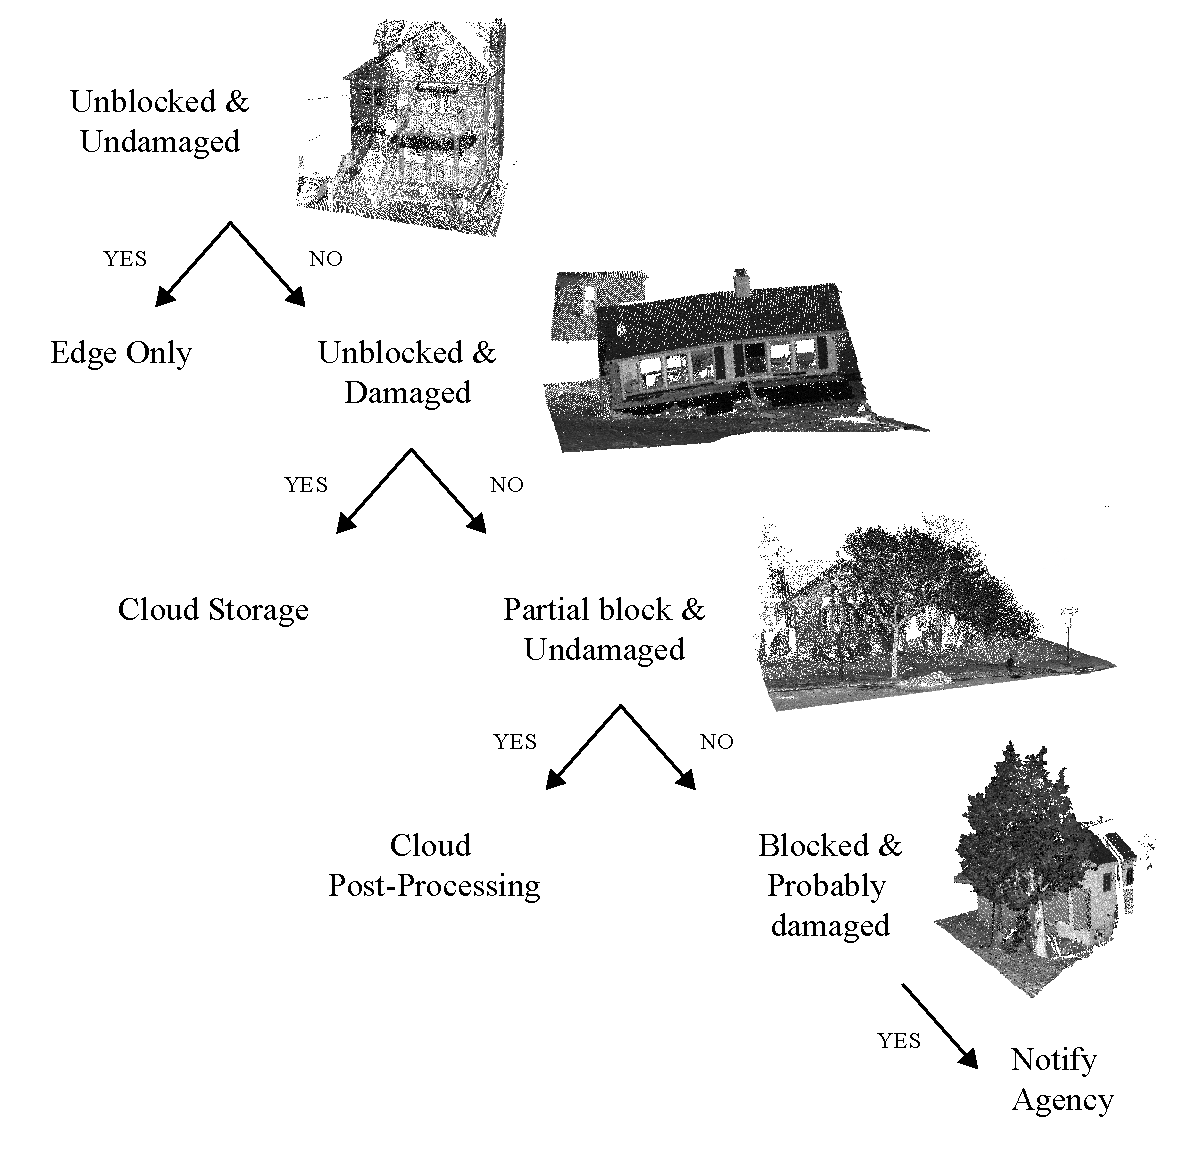
\includegraphics[width=0.5\linewidth]{Figures/diagonal.pdf}
  \caption{Disaster recovery decision stages and its associated reactions based on the LiDAR images.}
  \label{data_uncertainty}
\end{figure}

This workflow presents a content-driven stage where the stream-processing engine needs to perform decisions based on the content of the data that is being processed. Figure \ref{data_uncertainty} depicts all the different content-driven stages that our workflow presents in a decision tree way and its associated reactions. 

The workflow consists of multiple different stages driven by the content of the data (more data content variety means more stages), but only two of them need stream-processing capabilities. The first stage with stream-processing needs is where data gets generated and pre-processed; this stage is performed at the edge of the network so we can quickly and efficiently determine whether the building conditions are safe or not for evacuees to return. Depending on the results from this stage, we trigger the rest of the stages. The second stage, that also needs stream processing, is the change detection application which is executed in the cloud.

\subsubsection{Stage 1: Data generation - Pre-processing Stage}
The following are the actual pre-processing stages that we implemented in Apache Storm to determine the  conditions of the buildings.

\noindent\textbf{Noise Filtering:} flags or removes noise points in the LiDAR data.
\\
\noindent\textbf{Ground Point Classification:} it classifies the LiDAR points into ground object points and non-ground object points.
\\
\noindent\textbf{Classification:} it classifies the point features according to the geometry information. 
\\
\noindent\textbf{Visual inspection:} is designed to provide visual inspection, which allows experts or agencies to access the data and perform visual inspections and help perform more informed decisions.
\\
\noindent\textbf{Content-driven stage:} the last stage on the workflow is a content-driven stage where, depending on the results of the data, we might need to react and trigger further processing to determine if a building is safe or not for evacuees to return. The decision of whether or not data needs post-processing is based on two metrics obtained from the first stage of the pre-processing workflow. The two metrics are: data quality and computation intensity. 
\\
\\
Measurement of data quality: 
\begin{equation}
DQ=\frac{Spacing}{step\_para}\\
\end{equation}
where \textit{Spacing} represents the average edge length (2D) to all neighbor points of the original LiDAR data and \textit{step\_para} represents to the cell size (or the grid size) parameter of the grid-based interpolation.\\
\\
Measurement of computation intensity: 
\begin{equation}
CI=\frac{FileSize}{(X\_lowe - X\_upper) \cdot (Y\_lowe - Y\_upper)}
\end{equation}
\\
\noindent If both the data quality and the computation intensity do not satisfy the specified threshold then further processing is required and the second stage will be performed. 

Since this first stage will be performed at the edge of the network with limited computation capabilities, the user needs to have the ability to specify QoS metrics. In this case the user has the ability to specify a deadline that all the tuples have to meet, as one wants to get the results as fast as possible. 

The following mathematical expressions are the task optimization model proposed for this workflow:
\begin{equation}
\begin{split}
\max \sum x_{ij}
\\
\sum t_{ij} \cdot x_{ij} \leq t_{constraint} , \forall i
\\
x_{ij} \in {0,1}, \forall i,j
\end{split}
\end{equation}

\noindent Where $x_{ij}$ detonates the $j$th tasks at the processing level $i$. $x_{ij} \in {0,1}$ where $x_{ij} = 1$ indicates the execution of the process, while $x_{ij} = 0$ represents not executing the process. $t_{ij}$ denotes the estimated runtime of task $x_{ij}$. $t_{constraint}$ is the total workload budget for all tasks at level $i$.

\subsubsection{Stage 2: Change detection - Post-processing stage}
The following are the actual post-processing stages that we implemented and are triggered based on the content of the data.

\noindent\textbf{Historical data:} the first decision process to determine whether the data that needs further processing has any geo-spatial overlaps with the historical data that is currently stored in the system.

\noindent\textbf{Change detection:} the process that involves comparing changes between LiDAR photographs taken over different time periods that cover the exact same geographic area to understand how a given area has changed between two time periods. 

\noindent\textbf{Content-driven stage:} this stage will notify agencies if the results produced are alarmingly atrocious. 
\\
\\
\noindent To simulate this workflow we used real LiDAR images that were taken right after Hurricane Sandy struck back in 2012 in the NY and Long Island area, with a total of 741 images and 3.7 GB in size, with the biggest image size of 33.8 MB, and the smallest of 1.8 KB. For the historical data in stage 2 we used a bigger data set of pre-Hurricane Sandy. Supporting workflows that generate such large amounts of information at the edge of the network and having to transfer data back and forth between the edge and the core can prevent an effective reaction to an emergency situation and/or target application objectives.


\subsection{Scientific Observatory}

It's a networked ocean research observatory with arrays of instrumented water column moorings and buoys, profilers, gliders, and autonomous underwater vehicles within the different open ocean and coastal regions. OOI infrastructure also includes a cabled array of instrumented seafloor platforms and water column moorings on the Juan de Fuca tectonic plate. This networked system of instruments, moored and mobile platforms, and arrays provide ocean scientists, educators, and the public the means to collect sustained, time-series data sets to enable the examination of complex, interlinked physical, chemical, biological, and geological processes operating throughout the coastal regions and open ocean. OOI implements a geographically distributed, secure, highly available CI that is responsible for data acquisition/collection, data storage and processing, and on-demand delivery of data and data products to scientists and application developers. The use of a well-defined API based on standard protocols enables other systems to interface and interact with OOI CI programmatically. The scientific observatory use case has a similar problem to the disaster recovery use case where the data is to big to send to the cloud in order to offer real-time data delivery.

\subsection{Video Analytics} 

The last use case is the use of video analytics~\cite{8358733} for safety and security. In video analytics, a single video camera can produce about 25-30 frames/second. In HD and FHD cameras an 8-bit uncompressed RGB frame amounts to about 553 Mbps and 1.24 Gbps for a one minute video, respectively. With the advent of 4k and 3D video cameras, this size is likely to grow exponentially. Developers and engineers are facing the challenge of providing on-time analytics of video data to support public safety and security from video cameras. Cloud computing is not efficient enough to support prompt analytics of such video data~\cite{7488250}. Video Analytics based on edge computing is the only feasible approach to cater to low latency requirement for large-scale video streams~\cite{8057318}.

\subsection{Observe Orient Decide Act Loop}

The \ac{OODA} loop refers to the decision-making cycle of observe, orient, decide, and act, developed by military strategists and the United States Air Force~\cite{OODA}. \ac{OODA} is a decision-making cycle to process data streaming from sensors in real time, becoming an essential design characteristic for IoT applications. 
\begin{figure}[h!]
  \centering
  \includegraphics[width=0.8\columnwidth]{Figures/ooda.pdf}
  \caption{RIoTBench IoT high-level logical interactions between different sensors, applications and users.}
  \label{fig:etl}
\end{figure}

Anshu \textit{et al.}~\cite{RIoTBench} offer a suite of IoT applications that follows the closed-loop \ac{OODA} cycle. The applications are based on common IoT patterns for data pre-processing, statistical summarization, and predictive analytics. These are coupled with workloads sourced from real IoT observations. A high-level overview of the logical interaction of the IoT applications is depicted in Figure~\ref{fig:etl}.

\textbf{Extract-Transform-Load (ETL)} consumes data from hundreds of thousands of edge sensors, and pre-processes, cleans, and archives the data. Further, the results are published to an edge broker so that clients interested in real-time monitoring can subscribe to it, while a copy is forked to the cloud for storage, and another to the next dataflow step.

\textbf{Statistical Summarization (STATS)} performs higher order aggregation and plotting operations, and stores the generated plots into the cloud, from where webpages can load the visualization files on browsers. 

\textbf{Model Training (TRAIN)} periodically loads the stored data from ETL step and trains forecasting models that are stored in the cloud, and notifies the message broker of an updated model being available. 

\textbf{The Predictive Analytics (PRED)} subscribe to the message broker and downloads the new models from the cloud, and continuously operates over the pre-processed data stream from ETL to make predictions and classifications that can indicate actions to be taken on the domain. It then notifies the message broker of the predictions, which can independently be subscribed to by a user or device for action. 

The ETL dataflow requires a low-latency cycle in order to achieve real-time monitoring, in addition it also requires some of its operators to be located in the cloud for storing messages and others to be at the edge of the network. This makes the ETL workflow the perfect candidate workflow for testing the operator placement strategy proposed. 